% !TEX program = lualatex
\documentclass[11pt]{article}

% -------- LuaLaTeX : polices et langue --------
\usepackage{fontspec}
\setmainfont{Latin Modern Roman}
\setsansfont{Tex Gyre Heros}
%\renewcommand{\familydefault}{\sfdefault} % force le sans serif par défaut
\usepackage{polyglossia}
\setdefaultlanguage{french}

% -------- Mise en page --------
\usepackage[a4paper,margin=1cm]{geometry}
\usepackage{multicol}
\usepackage{fancyhdr}
\pagestyle{empty}
\usepackage[most]{tcolorbox}

% -------- Mathématiques --------
\usepackage{amsmath,amssymb,mathtools}
\usepackage{icomma}
% \sisetup{locale=FR}

\usepackage{enumitem}
\setlist[itemize]{left=0pt}
\setlist[enumerate]{left=0pt, label=\textbf{\arabic*}.}

\usepackage{ProfCollege}
\usepackage{ProfMaquette}

\usepackage{tabularray}

% -------- Divers --------
\setlength{\parindent}{0pt}

\begin{document}

\begin{Maquette}[Fiche]{Theme=Translations, Niveau=Quatrième}

\begin{exercice}
    \begin{center}
    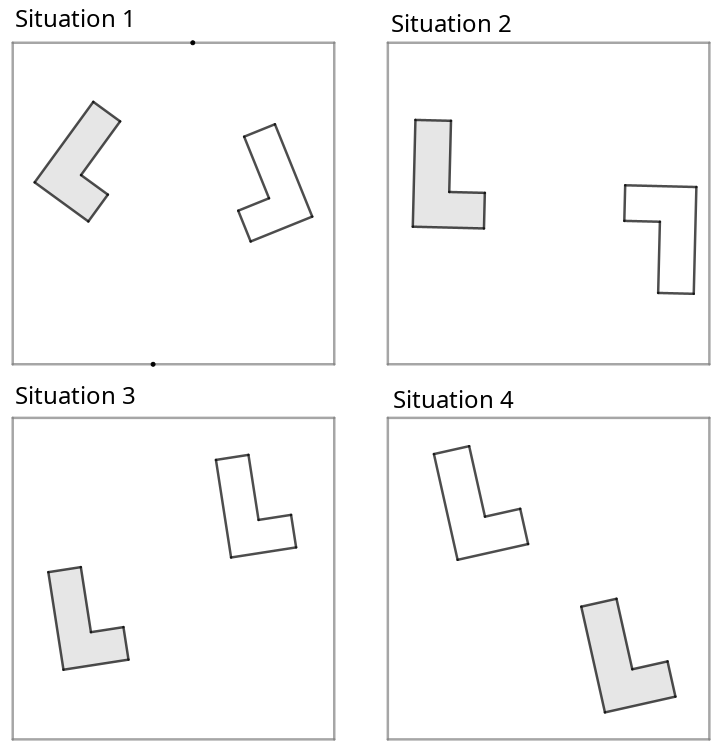
\includegraphics[width=.75\linewidth]{Images/exercice1.png}
    \end{center}
    Dans chaque situation, la lettre L noire a été transformée géométriquement en la lettre blanche.
    \begin{enumerate}
        \item Quelles transformations ont été utilisées dans les situations 1 et 2 ?
        \item Et dans les situations 3 et 4 ?
    \end{enumerate}
\end{exercice}

\end{Maquette}

\end{document}
